\documentclass[a4paper,14pt]{extreport}

\usepackage[T1,T2A]{fontenc}
\usepackage[utf8]{inputenc}

\usepackage{style/bsumain}
\usepackage{style/bsucoursetitle}
\usepackage{blindtext}
\usepackage{hyperref}


\begin{document}
  
%  \begin{titlepage}
\begin{center}

%\large
\textbf{МИНИСТЕРСТВО ОБРАЗОВАНИЯ РЕСПУБЛИКИ БЕЛАРУСЬ}
\vspace{1.5 ex}

\textbf{БЕЛОРУССКИЙ ГОСУДАРСТВЕННЫЙ УНИВЕРСИТЕТ}
\vspace{1.5 ex}

\textbf{ФАКУЛЬТЕТ ПРИКЛАДНОЙ МАТЕМАТИКИ И ИНФОРМАТИКИ}
\vspace{1.5 ex}

\textbf{Кафедра дискретной математики и алгоритмики}
\vspace{7 ex}

\noindent
ГУЛИН

\large
Кирилл Иванович
\vspace{5 ex}

$ $

$ $

$ $


\textbf{ИССЛЕДОВАНИЕ МЕТОДОВ ВЫДЕЛЕНИЯ СМЫСЛОВЫХ ЕДИНИЦ ИЗ ДЕЛОВОЙ ПЕРЕПИСКИ}

\vspace{7 ex}
\large
Дипломная работа
\vspace{5 ex}

\begin{tabbing}
\hspace*{107mm}\=\hspace*{7cm}
\kill 
 \> Научный руководитель: \\
 \>  доцент Ю. В. Свирид \\ \vspace{5 ex}

Допущен к защите \\
<<\rule {30pt} {0.5 pt}>>\rule {100pt} {0.5 pt} 2021 г. \> \\
Зав. кафедрой дискретной математики \> \\
и алгоритмики, доктор физ.-мат. наук,\> \\
профессор В. М. Котов
\end{tabbing}

\vfill

$ $

Минск, 2021

\end{center}

\end{titlepage}
  
  

%  \maketitle


  \setcounter{page}{2}

  {
    \renewcommand{\contentsname}{Содержание}
    \tableofcontents
  } 
 
  \chapter*{РЕФЕРАТ}

Дипломная работа, 33 с., 23 рис., 12 источников.

Ключевые слова: ОБРАБОТКА ТЕКСТОВ, МАШИННОЕ ОБУЧЕНИЕ, ЛАТЕНТНОЕ РАЗМЕЩЕНИЕ ДИРИХЛЕ, МЕТОДЫ ПОНИЖЕНИЯ РАЗМЕРНОСТИ, ВЕКТОРНОЕ ПРЕДСТАВЛЕНИЕ ТЕКСТОВ, СТАТИСТИЧЕСКИЙ АНАЛИЗ, МЕТОДЫ КЛАСТЕРИЗАЦИИ, НЕЙРОННЫЕ СЕТИ.

\vspace{1.5 ex}
Объект исследования --- наборы данных деловых электронных переписок. 

Цель работы --- анализ деловых электронных переписок методами машинного обучения.

Методы исследования --- латентное размещение Дирихле, методы кластеризации, методы обработки текстов, методы понижения размерности, методы получения векторных представлений.

Работа посвящена исследованию и анализу деловых электронных переписок, в частности, переписок Хиллари Клинтон и переписок сотрудников корпорации Enron. В результате работы был произведен статистический анализ электронных переписок. Были обнаружены закономерности в исходных данных. Также была разработана кластеризация содержаний электронных писем, в результате которой получились интерпретируемые результаты, что показало эффективность разработанных методов.
 


%%%%%%%%%%%%%%%%%%%%%%%%%%%%%%%%%%%%%%%%%%%%%%%%%%%%%%%%%%%
\chapter*{РЭФЕРАТ}

Дыпломная праца, 33 с., 23 рыс., 12 крыніц.

Ключавыя словы: АПРАЦОЎКА ТЭКСТАЎ, МАШЫННАЕ НАВУЧАННЕ, ЛАТЭНТНАЕ РАЗМЯШЧЭННЕ ДЫРЫХЛЕ, МЕТАДЫ ЗНІЖЭННЯ ПАМЕРНАСЦІ, ВЕКТАРНАЕ ПРАДСТАЎЛЕННЕ ТЭКСТАЎ, СТАТЫСТЫЧНЫ АНАЛІЗ, МЕТАДЫ КЛАСТАРЫЗАЫІ, НЕЙРОНАВЫЯ СЕТКІ.

Аб'ект даследавання --- наборы дадзеных дзелавых электронных перапісак.

Мэта работы --- аналіз дзелавых электронных перапісак метадамі машыннага навучання.

Метады даследавання --- латэнтнае размяшчэнне Дырыхле, метады кластарызацыі, метады апрацоўкі тэкстаў, метады зніжэння памернасці, метады атрымання вектарных уяўленняў.

Праца прысвечана даследаванню і аналізу дзелавых электронных перапісак, у прыватнасці, перапісак Хілары Клінтан і перапісак супрацоўнікаў карпарацыі Enron. У выніку працы быў выраблены статыстычны аналіз электронных перапісак. Былі выяўлены заканамернасці ў зыходных дадзеных. Таксама была распрацавана кластарызацыя зместаў электронных перапісак, у выніку якой атрымаліся інтэрпрэтаваныя вынікі, што паказала эфектыўнасць распрацаваных метадаў.


%%%%%%%%%%%%%%%%%%%%%%%%%%%%%%%%%%%%%%%%%%%%%%%%%%%%%%%%%%%

\chapter*{ABSTRACT}

Diploma thesis, 33 p., 18 fig., 12 sources.

Keywords: TEXT PROCESSING, MACHINE LEARNING, LATENT DIRICHLET ALLOCATION, DIMENSION REDUCTION METHODS, TEXT EMBEDDINGS, STATISTICAL ANALYSIS, CLUSTERIZATION METHODS, NEURAL NETWORKS.

\vspace{1.5 ex}
The object of research is business e-mail datasets.

Objective: analysis of business e-mails using machine learning methods.

Research methods --- latent Dirichlet allocation, clustering methods, text processing methods, dimension reduction methods, methods for obtaining text embeddings.

The work is devoted to the research and analysis of business e-mails, in particular, the e-mails of Hillary Clinton and the e-mails of employees of the Enron corporation. As a result of the work, a statistical analysis of emails was carried out. Patterns were found in the original data. Also, the clustering of the contents of e-mails was developed, as a result of which interpretable results were obtained, which showed the effectiveness of the developed methods.

  
  \chapter*{Введение}

С ростом доступности электронных документов и быстрым ростом всемирной паутины задача автоматической категоризации документов стала ключевым cпособом классификации и группирования информации и знаний любого рода. Для правильной классификации электронных документов, онлайн-новостей, блогов, электронной почты и электронных библиотек необходимы интеллектуальный анализ текста (англ. \textit{Text Mining}), машинное обучение (англ. \textit{Machine Learning}) и методы обработки текстов на естественном языке (англ. \textit{Natural Language Processing, NLP}).

Современные системы обработки текстов на естественном языке
могут анализировать неограниченные объемы текстовых данных. Они могут понимать суть сложных контекстов, расшифровывать двусмысленности языка, извлекать ключевые факты и взаимосвязи. Учитывая огромное количество неструктурированных данных, которые создаются каждый день, от электронных медицинских карт до сообщений в социальных сетях, обработка текстов на естественных языках стала критически важной для эффективного анализа текстовых данных.


\addcontentsline{toc}{chapter}{Введение}
\clearpage

 
  \chapter{Используемые данные}

\section{Электронные письма Хиллари Клинтон}

В 2015 году Хиллари Клинтон (американский политик, государственный секретарь США в 2009-2013 гг., кандидат в президенты США в 2016 г.) была вовлечена в большое количество споров по поводу использования личных учетных записей электронной почты на негосударственных серверах во время ее пребывания на посту государственного секретаря США. Некоторые политические эксперты утверждают, что использование Клинтон личных учетных записей электронной почты для ведения дел госсекретаря является нарушением протоколов и федеральных законов, обеспечивающих надлежащий учет деятельности правительства. 



Был подан ряд исков о свободе информации из-за того, что Государственный департамент США не опубликовал полностью электронные письма, отправленные и полученные на личные аккаунты Клинтон. На сегодняшний день Государственным департаментом США опубликовано почти 7000 страниц отредактированных электронных писем Клинтон. 

Документы были опубликованы в формате PDF. Платформа \textit{Kaggle} очистила и нормализовала выпущенные документы и разместила их для публичного анализа. Мы будем основываться именно на датасете, опубликованном \textit{Kaggle}.

\section{Исследования, проведенные над наборами данных}

\subsection{Исследования над письмами Хиллари Клинтон}


Анализ, проведенный центром Беркмана Кляйна по интернету и обществу в Гарвардском университете и центром Шоренштейна в Гарвардской школе Кеннеди, показывает, что споры по поводу электронной почты Клинтона получили больше освещения в основных средствах массовой информации, чем любая другая тема во время президентских выборов США 2016 года \cite{clinton_research_bib}.

Например, исследование профессора Уэйн Олдфорда и студента бакалавра университета Уотерлу построили инструмент для анализа содержимого писем \cite{clinton_oldford_bib}.

Инструмент предоставляет визуальные аналитические инструменты и демонстрирует, как много можно узнать о человеке из того, что ошибочно считается неинформативными метаданными. По словам Олдфорда, <<общественность может воспроизвести наши анализы и сама увидеть, как они могут быть показательными, особенно в сочетании с другими общедоступными источниками>>.

Например, приложение показывает ежедневный объём электронной почты, отправленной и полученной Клинтон, а также слова, наиболее часто встречающиеся в электронных письмах за выбранный период времени.

Например, при анализе данных исследователи обнаружили 10 периодов отсутствия электронных писем от Клинтон, пока она была госсекретарем, включая значительный разрыв между 30 октября и 9 ноября 2012 года, который совпадает с первоначальным расследованием нападения в Бенгази и его последствий, а также президентских выборов в США в 2012 году.

Существует большое количество исследований электронных писем Клинтон, выполненные пользовалями $Kaggle$. К сожалению, качество данных работ не является высоким, поскольку они, во-первых, не являются большими проектами, а представляют собой скорее любительские исследования, а во-вторых, при этом часто выполнены с недостатками, например, с плохой предобработкой исходных данных. 


\subsection{Исследования над письмами корпорации Enron}

По крайней мере два исследования, касающихся классификации текстов, были выполнены на наборе данных \textit{Enron}. Один из них --- автоматическая категоризация электронной почты по папкам, выполняемая факультетом компьютерных наук Массачусетского университета \cite{bib_5}. Другой связан с анализом социальных сетей. Используя корпус \textit{Enron} и судебные документы, выпущенные судом США по делам о банкротстве, Джитеш Шетти и Джафар Адиби извлекли из электронной почты социальную сеть, состоящую из 151 сотрудника, соединив людей, которые обменивались электронными письмами \cite{bib_6}.

Кроме того, команда \textit{Legal Track} конференции по извлечению текстов (<<\textit{Text Retrieval Conference Legal Track}>>) фокусировалась на методах крупномасштабного поиска текста. Команда ученых изучала следующие методы поиска: булевы, нечеткие модели поиска, вероятностные (байесовские) модели, статистические методы, подходы машинного обучения, инструменты категоризации и анализ социальных сетей. Исследователи \textit{TREC Legal Track}
пришли к выводу, что «всего от 22 до 57 процентов релевантных документов могут быть извлечены с помощью различных альтернативных методов поиска».

В статье Шетти и Адиби набор данных \textit{Enron} использовался для классификации электронной почты на основе моделирования энтропии графа. Энтропия пыталась выбрать наиболее интересные вершины в графе, вершины которого представляют электронные письма, а ребра --- сообщения между пользователями \cite{bib_7}.

Что касается непосредственно тематического моделирования и кластеризации, проводимых в данной работе, основная масса исследований представлена небольшими проектами, выполненными пользователями \textit{Kaggle}. Как и в случае с электронными письмами Клинтон, в силу аналогичных причин, качество данных работ не является высоким.



\newpage


  \chapter{Обзор используемых технологий}

\section{BERTopic}

BERTopic -- это метод моделирования тем, который использует трансформеры и c-TF-IDF для создания плотных кластеров, позволяющих легко интерпретировать темы, сохраняя при этом важные слова в описаниях тем \cite{bib234234}. 

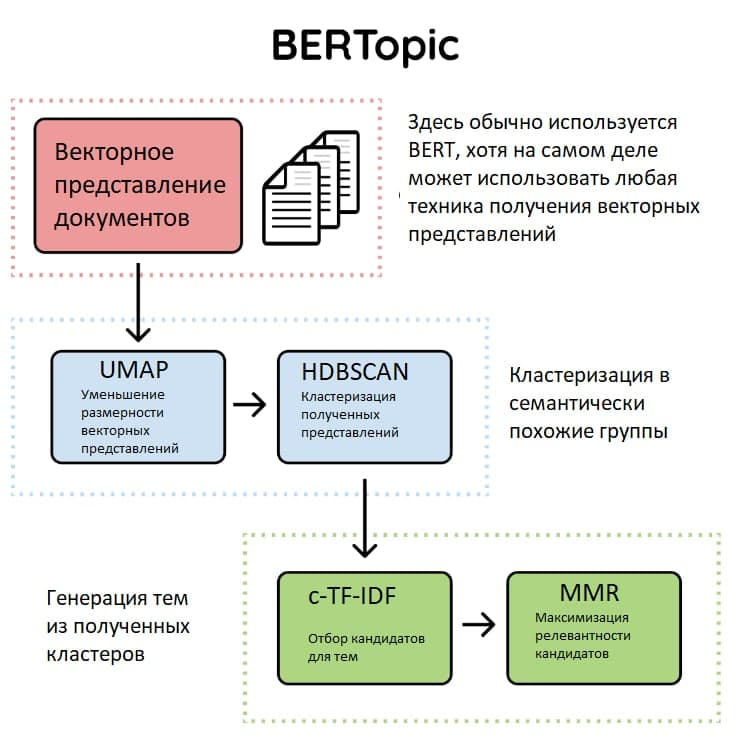
\includegraphics[scale=0.9]{pics/bertopic.jpg}


Первый шаг, который нам нужно сделать -- это преобразовать документы в числовые данные. Для этой цели мы используем BERT, поскольку он извлекает различные векторные представления слов в зависимости от контекста. Это одна из лучших моделей в настоящее время для многих задач, связанных с текстом. BERT получил награду за лучшую работу на ежегодной конференции североамериканского отделения  компьютерной лингвистики 2019 года \cite{bib_1} \cite{bib_2}.

Мы хотим убедиться, что документы с похожим смыслом сгруппированы вместе, чтобы мы могли найти темы в этих кластерах. Перед этим нам сначала нужно снизить размерность векторных представлений слов, поскольку многие алгоритмы кластеризации плохо справляются с высокой размерностью. 
UMAP -- это один из немногих алгоритмов уменьшения размерности, он является наиболее эффективным,
 поскольку он сохраняет значительную часть многомерной локальной структуры в более низкой размерности. 


После уменьшения размерности встраиваемых документов  мы можем кластеризовать документы с помощью HDBSCAN (Hierarchical Density-Based Spatial Clustering of Applications with Noise).
HDBSCAN основан на алгоритме DBSCAN и, как и другие алгоритмы кластеризации, используется для группировки данных \cite{bib_3}.

Помимо того, что он обычно показывает лучшее качество, он также быстрее, чем обычный DBSCAN. Ниже приведен график нескольких алгоритмов кластеризации. При отметке в 200 000 объектов DBSCAN занимает примерно вдвое больше времени, чем HDBSCAN. Стоит отметить, что по мере увеличения количества объектов разница в производительности будет и дальше увеличиться в пользу HDBSCAN:
\newline

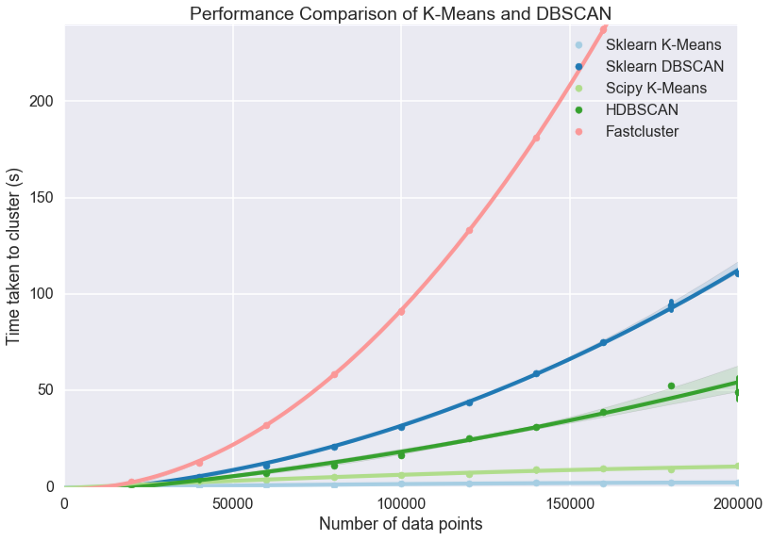
\includegraphics[scale=0.5]{pics/clustering-comparison.png}



HDBSCAN алгоритм кластеризации, который довольно хорошо работает с UMAP, поскольку UMAP поддерживает большую локальную структуру даже в пространстве меньшей размерности. Более того, HDBSCAN не переносит отдельные точки в кластеры, поскольку считает их выбросами.


Теперь мы сгруппировали похожие документы вместе, которые должны представлять темы, из которых они состоят. Что мы хотим узнать из созданных нами кластеров -- это то, что отличает один кластер по своему содержанию от другого.  Как мы можем извлечь темы из сгруппированных документов? Чтобы решить эту проблему, используется классовый вариант TF-IDF (c-TF-IDF), который позволил бы извлечь то, что делает каждый набор документов уникальным по сравнению с другим. Интуиция, лежащая в основе метода, заключается в следующем: когда мы применяем TF-IDF как обычно к набору документов, мы в сравниваем важность слов среди всех документов, а в классовом варианте теперь у нас есть одно значение важности для каждого слова в кластере, которое можно использовать для создания темы. Если мы возьмем несколько  самых важных слов в каждом кластере, то получим хорошее представление о кластере и, следовательно, теме.

Чтобы создать эту оценку классового TF-IDF, нам нужно сначала создать один документ для каждого кластера документов:

\begin{verbatim}
docs_df = pd.DataFrame(data, columns=["Doc"])
docs_df['Topic'] = cluster.labels_
docs_df['Doc_ID'] = range(len(docs_df))
docs_per_topic = docs_df.groupby(['Topic'], as_index = False) \
.agg({'Doc': ' '.join})
\end{verbatim}

Затем мы применяем TF-IDF на основе классов:

\begin{center}
$\text{c-TF-IDF}_{i} = 
\dfrac{t_i}{w_i} \cdot 
\log{
\dfrac{m}{\sum\limits_j^n t_j}}$
\end{center}

Где частота каждого слова $t$ извлекается для каждого класса $i$ и делится на общее количество слов $w$ в классе. Это действие можно рассматривать как форму регуляризации частых слов в классе. Затем общее количество документов $m$ делится на общую частоту слова $t$ по всем $n$ классам.

Теперь у нас есть одно значение важности для каждого слова в кластере, которое можно использовать для создания темы. После обучения нашей модели мы можем итеративно пройти, возможно, сотню тем, чтобы получить хорошее представление о темах, которые были извлечены. Однако это занимает некоторое время и не имеет глобального представления. Вместо этого мы можем визуализировать темы. Для этого используется представление тем в 2D с помощью UMAP, а затем визуализируем два измерения с помощью графического представления, чтобы мы могли создать интерактивное представление. Пример визуализации от авторов алгоритма:
% https://maartengr.github.io/BERTopic/tutorial/visualization/visualization.html

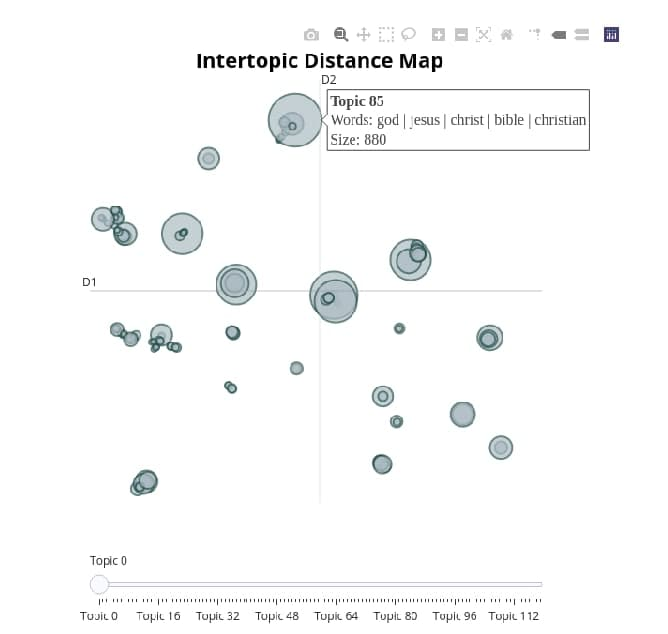
\includegraphics[scale=0.9]{pics/bertopic-visual-1.jpg}

На картинке видно, что кластеры довольно равномерно распределились по пространству и кластера действительно очень интерпремируемы: например, на рисунке показан кластер религиозных слов.


Мы также можем рассчитать вероятность того, что темы могут быть найдены в документе. Эти вероятности означают, насколько BERTopic уверен в том, что определенные темы могут быть найдены в документе:
% https://maartengr.github.io/BERTopic/tutorial/visualization/visualization.html

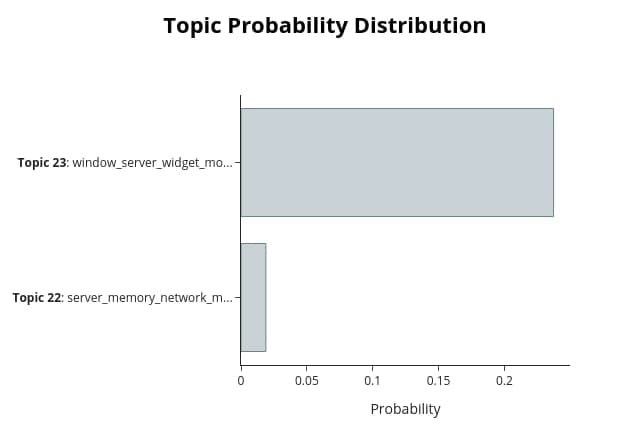
\includegraphics[scale=0.9]{pics/bertopic-visual-2.jpg}

Важно понимать, что распределение вероятностей не указывает на распределение частотности тем в документе. Это просто показывает, насколько BERTopic уверен в том, что в документе можно найти определенные темы.


  \chapter{Обзор используемых технологий}

\section{Тематическое моделирование}

Тематическое моделирование --- это метод классификации документов, аналогичный кластеризации по числовым данным, который находит некоторые естественные группы элементов (темы), даже в случаях, когда пользователь не имеет конкретной цели касательно нахождения определенных тем.

Документ может быть частью нескольких тем, как в нечеткой (мягкой) кластеризации, в которой каждый элемент данных принадлежит более чем одному кластеру.

Тематическое моделирование предоставляет методы для автоматической организации, понимания, поиска и обобщения больших электронных архивов. Это может помочь в следующих случаях:

\begin{itemize}
\item обнаружение скрытых (неочевидных) тем в корпусе (т.е. общем наборе слов) данных,
\item классификация документов по обнаруженным темам,
\item использование классификации для, собственно, организации, обобщения либо поиска интересующих документов.
\end{itemize}

Например, предположим, что документ относится к темам \textit{еда}, \textit{собаки} и \textit{здоровье}. Таким образом, если пользователь запрашивает <<\textit{корм для собак}>>, вышеупомянутый документ может определиться как релевантный, поскольку, помимо других тем, он охватывает и эти темы. Другими словами, его релевантность по отношению к запросу может быть выяснена даже без просмотра всего документа, а только на основании уже известных тем.

Получается, аннотируя документ на основе тем, предсказанных методом моделирования, становится возможно оптимизировать выполняемый процесс поиска.

\section{Предобработка электронных писем корпорации Enron}

\subsection{Выделение метаданных из сырого текста писем}

Набор данных \textit{Enron} также требует предварительной обработки. К примеру, так выглядит необработная информация одного электронного письма:

\begin{verbatim}
Message-ID: <18782981.1075855378110.JavaMail.evans@thyme>
Date: Mon, 14 May 2001 16:39:00 -0700 (PDT)
From: phillip.allen@enron.com
To: tim.belden@enron.com
Subject: 
Mime-Version: 1.0
Content-Type: text/plain; charset=us-ascii
Content-Transfer-Encoding: 7bit
X-From: Phillip K Allen
X-To: Tim Belden <Tim Belden/Enron@EnronXGate>
X-cc: 
X-bcc: 
X-Folder: \\Phillip_Allen_Jan2002_1\\Allen, Phillip K.\\\'Sent Mail
X-Origin: Allen-P
X-FileName: pallen (Non-Privileged).pst

Here is our forecast
\end{verbatim}

Конечно, анализировать данные (в том числе метаинформацию о письме) в таком формате бессмысленно. Для обработки мы будем использовать библиотеку \textit{email} \cite{bib8}. Данная библиотека позволяет из сырых данных выделить вспомогательную информацию о письме, в частности, библиотека позволяет выделить следующие интересные нам атрибуты:
\begin{itemize}
\item полное содержание письма,
\item дата отправки,
\item адрес получателя,
\item адрес отправителя,
\item тема письма,
\item логин отправителя.
\end{itemize}

\subsection{Выделение содержания писем}

После этого требуется также привести содержание письма в приемлимый для дальнейшего обучения вид. Например, для письма с содержанием ниже мы хотим выделить только единицы, имеющие отношение к сути письма.

\begin{verbatim}

Forwarded by Phillip K Allen/HOU/ECT on 09/12/2000 11:22 AM 

Michael Etringer

09/11/2000 02:32 PM

To: Phillip K Allen/HOU/ECT@ECT
cc:  
Subject: Contact list for mid market

Phillip,
Attached is the list. Have your people fill in the columns 
highlighted in yellow. As best can we will try not to overlap
on accounts. 
Thanks, Mike
\end{verbatim}

Выделение этих единиц происходит в соответствии со следующей последовательности шагов:
\begin{enumerate}
\item Перевод всех символов в нижний регистр.
\item Удаление всех слов, содержащих цифры. Такие слова не несут смысловой нагрузки и, соответственно, влияют на качество обучения в худшую сторону (подавляющее большинство таких слов было получено отправителями по ошибке).
\item Удаление единиц, соответствующих информации о пересланных письмах.
\item Удаление единиц, соответствующих информации о вложениях в письме.
\item Удаление единиц, соответствующих почтовым адресам, присутствующим в тексте писем.
\item Удаление единиц, соответствующих корпоративным именам пользователей.
\item Удаление единиц, соответствующих ссылкам в сети Интернет.
\item Удаление единиц, не несущих смысловой составляющей, в заголовке письма.
\end{enumerate}

Шаги 3-7 выполняются с использованием регулярных выражений. 

В результате, для примера выше, дальнейшая работа будет производиться со следующим текстом:
\begin{verbatim}
contact list for mid market. phillip, attached is the list. 
have your people fill in the columns highlighted in yellow. 
as best can we will try not to overlap on accounts. thanks, mike'
\end{verbatim}




\section{BERTopic}

\textit{BERTopic} --- это метод моделирования тем, который использует трансформеры и \textit{c-TF-IDF} для создания плотных кластеров, позволяющих легко интерпретировать темы, сохраняя при этом важные слова в описаниях тем \cite{bib234234}. 

\subsection{Алгоритм}

\begin{figure}[H]
\centering
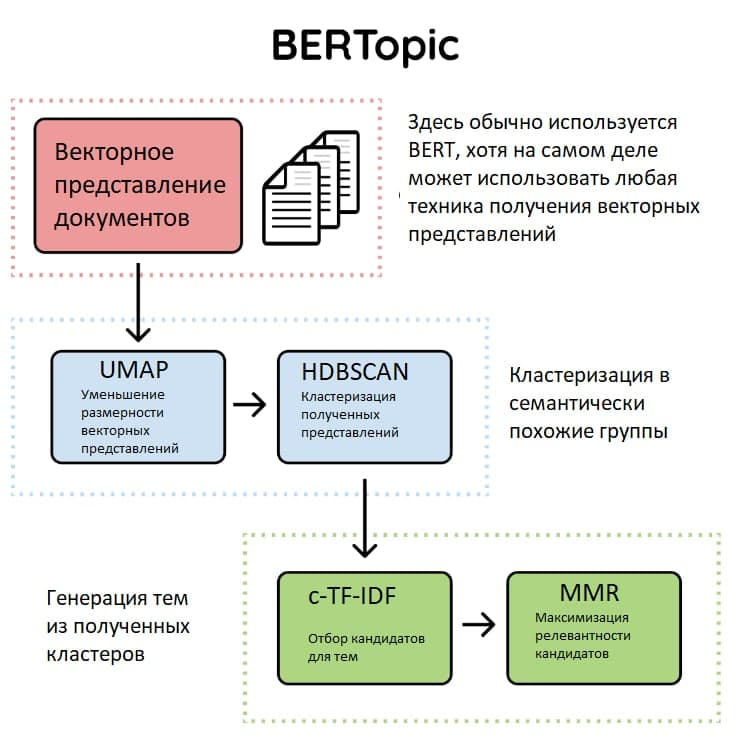
\includegraphics[scale=0.7]{pics/bertopic.jpg}
\caption{Стадии работы алгоритма \textit{BERTopic}}
\end{figure}

Алгоритм состоит из 3 шагов:

\begin{enumerate}

\item Первый шаг, который требуется сделать -- это преобразовать документы в числовые данные. Для этой цели используется \textit{BERT}, который извлекает различные векторные представления слов в зависимости от контекста. Это одна из лучших моделей в настоящее время для многих задач, связанных с текстом. \textit{BERT} получил награду за лучшую работу на ежегодной конференции североамериканского отделения  компьютерной лингвистики 2019 года \cite{bib_1} \cite{bib_2}.

\item Далее необходимо убедиться, что документы с похожим смыслом сгруппированы вместе, чтобы мы могли найти темы в этих кластерах. Перед этим нам сначала нужно снизить размерность векторных представлений слов, поскольку многие алгоритмы кластеризации плохо справляются с высокой размерностью. 
\textit{UMAP} --- это один из немногих алгоритмов уменьшения размерности, он является наиболее эффективным,
 поскольку он сохраняет значительную часть многомерной локальной структуры в более низкой размерности. 


После уменьшения размерности встраиваемых документов  мы можем кластеризовать документы с помощью \textit{HDBSCAN} (\textit{Hierarchical Density-Based Spatial Clustering of Applications with Noise}).
\textit{HDBSCAN} основан на алгоритме \textit{DBSCAN} и, как и другие алгоритмы кластеризации, используется для группировки данных \cite{bib_3}.

Помимо того, что он обычно показывает лучшее качество, он также быстрее, чем обычный 
\textit{DBSCAN}. Ниже приведен график нескольких алгоритмов кластеризации. При отметке в 200 000 объектов \textit{DBSCAN} занимает примерно вдвое больше времени, чем 
\textit{HDBSCAN}. Стоит отметить, что по мере увеличения количества объектов разница в производительности будет и дальше увеличиться в пользу \textit{HDBSCAN}:
\newline

\begin{figure}[H]
\centering
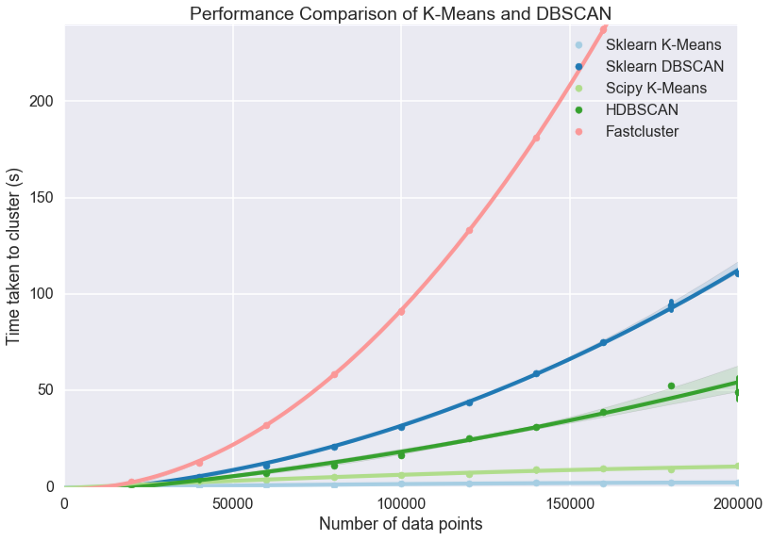
\includegraphics[scale=0.5]{pics/clustering-comparison.png}
\caption{Сравнение производительности алгоритмов кластеризации}
\end{figure}

\textit{HDBSCAN} --- алгоритм кластеризации, который довольно хорошо работает с 
\textit{UMAP}, поскольку \textit{UMAP} поддерживает большую локальную структуру даже в пространстве меньшей размерности. Более того, \textit{HDBSCAN} не переносит отдельные точки в кластеры, поскольку считает их выбросами.

\item Теперь мы сгруппировали похожие документы вместе, которые должны представлять темы, из которых они состоят. Что мы хотим узнать из созданных нами кластеров --- это то, что отличает один кластер по своему содержанию от другого.  Как мы можем извлечь темы из сгруппированных документов? Чтобы решить эту проблему, используется классовый вариант 
\textit{TF-IDF} (\textit{c-TF-IDF}), который позволил бы извлечь то, что делает каждый набор документов уникальным по сравнению с другим. Интуиция, лежащая в основе метода, заключается в следующем: когда мы применяем \textit{TF-IDF} как обычно к набору документов, мы в сравниваем важность слов среди всех документов, а в классовом варианте теперь у нас есть одно значение важности для каждого слова в кластере, которое можно использовать для создания темы. Если мы возьмем несколько  самых важных слов в каждом кластере, то получим хорошее представление о кластере и, следовательно, теме.

Чтобы создать эту оценку классового \textit{TF-IDF}, сначала нужно создать один документ для каждого кластера документов.
%\begin{verbatim}
%docs_df = pd.DataFrame(data, columns=["Doc"])
%docs_df['Topic'] = cluster.labels_
%docs_df['Doc_ID'] = range(len(docs_df))
%docs_per_topic = docs_df.groupby(['Topic'], as_index = False) \
%.agg({'Doc': ' '.join})
%\end{verbatim}
Затем мы применяем \textit{TF-IDF} на основе классов:

\begin{center}
$\textit{c-TF-IDF}_{i} = 
\dfrac{t_i}{w_i} \cdot 
\log{
\dfrac{m}{\sum\limits_j^n t_j}}$
\end{center}

Где частота каждого слова $t$ извлекается для каждого класса $i$ и делится на общее количество слов $w$ в классе. Это действие можно рассматривать как форму регуляризации частых слов в классе. Затем общее количество документов $m$ делится на общую частоту слова $t$ по всем $n$ классам.

Теперь у нас есть одно значение важности для каждого слова в кластере, которое можно использовать для создания темы. После обучения нашей модели мы можем итеративно пройти, возможно, сотню тем, чтобы получить хорошее представление о темах, которые были извлечены. Однако это занимает некоторое время и не имеет глобального представления. Вместо этого мы можем визуализировать темы. 

\end{enumerate}

\subsection{Интерпретация работы алгоритма} 

Для визуализации работы алгоритмы используется представление тем в 
\textit{2D} с помощью \textit{UMAP}, который создает двумерную проекцию всех точек и затем визуализирует эти два измерения, причем в интерактивном виде, что позволяет нам получить представление, понятное человеку. Пример визуализации от авторов алгоритма \cite{bib_4}:


\begin{figure}[H]
\centering
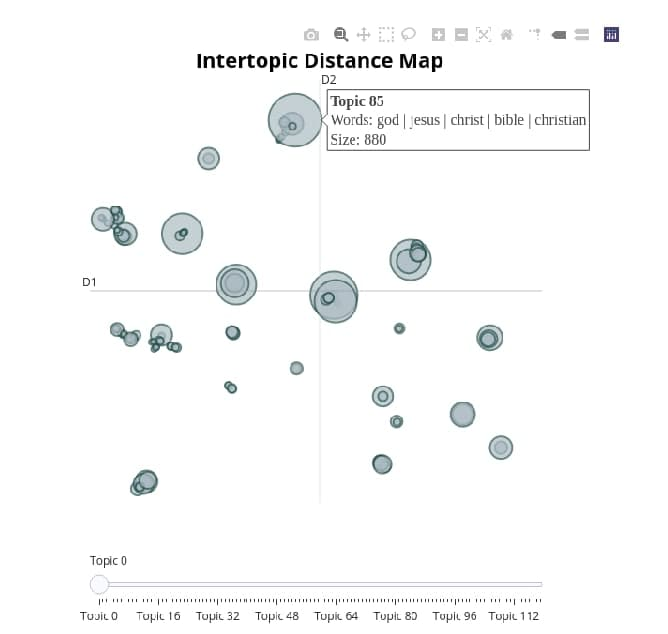
\includegraphics[scale=0.9]{pics/bertopic-visual-1.jpg}
\caption{Пример визуализации тем в $BERTopic$}
\end{figure}

На картинке видно, что кластеры довольно равномерно распределились по пространству и кластера действительно очень интерпремируемы: например, на рисунке показан кластер религиозных слов.

Мы также можем рассчитать вероятность того, что темы могут быть найдены в документе. Эти вероятности означают, насколько \textit{BERTopic} 
уверен в том, что определенные темы могут быть найдены в документе \cite{bib_4}:


\begin{figure}[H]
\centering
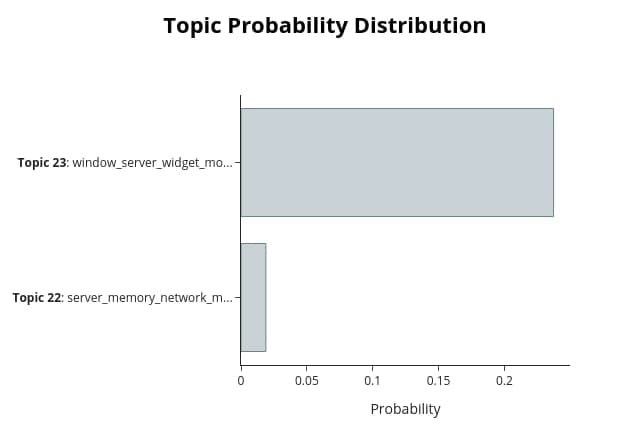
\includegraphics[scale=0.9]{pics/bertopic-visual-2.jpg}
\caption{Пример распределения вероятностей тем в $BERTopic$}
\end{figure}


Важно понимать, что распределение вероятностей не указывает на распределение частотности тем в документе. Это просто показывает, насколько 
\textit{BERTopic} уверен в том, что в документе можно найти определенные темы.

  
  \chapter{Анализ электронных писем}

Прежде чем приступать к исследованию данных методами машинного обучения, может быть полезно посмотреть на различного статистики.

\section{Анализ электронных писем Хиллари Клинтон}

\subsection{Количества слов}

\begin{itemize}

\item Гистограмма распределения количества слов каждой длины: 

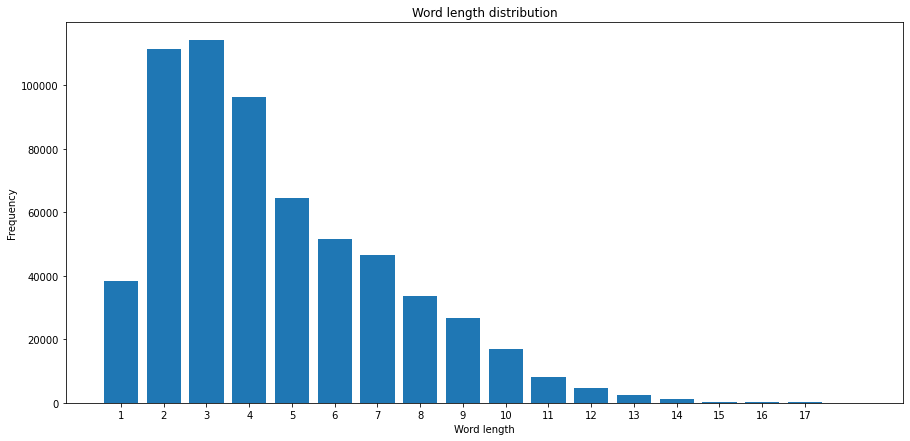
\includegraphics[scale=0.5]{pics/word_lengths.png}

Гистограмма выглядит вполне естественным образом, много коротких слов (например, местоимений, предлогов).

\item Гистограмма распределения длин (в количестве слов) писем:

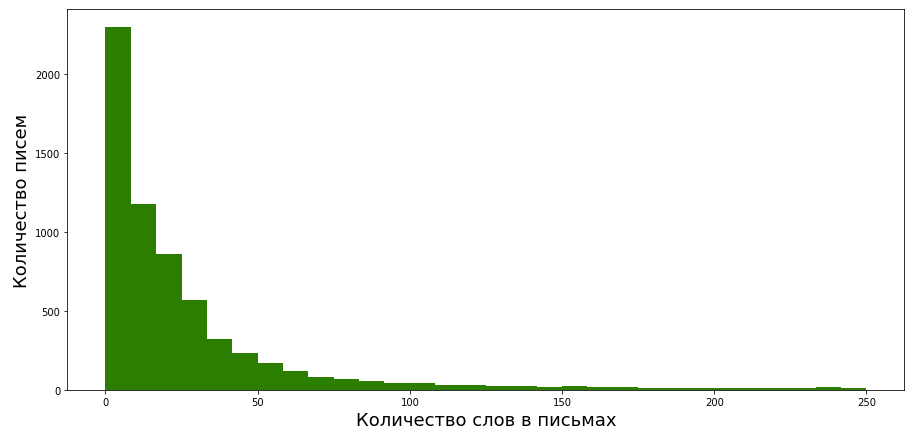
\includegraphics[scale=0.5]{pics/email_lengths.png}

Гистограмма соответствует интуитивным ожиданиям -- более длинные письма пишутся реже. 
\end{itemize}

\subsection{Время отправки писем}

\begin{itemize}

\item Количество отправленных писем по годам:

$ $

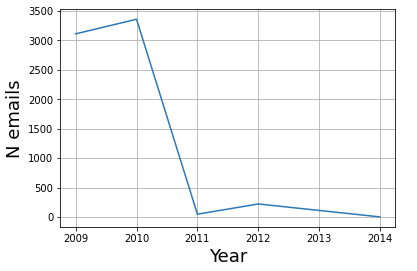
\includegraphics[scale=0.8]{pics/year.png}

На графике можно заметить странную аномалию с нулем писем в 2011 году. Вероятнее всего, это связано с особенностями набора данных. 

\item Количество отправленных писем по дням недели:

$ $

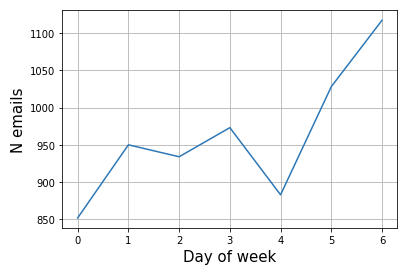
\includegraphics[scale=0.8]{pics/week.png}

График выглядит слегка неестественно (в отличие от \textit{Enron}). Можно попытаться интерпретировать это как особенности одного отдельного человека, занимающего специфичным видом деятельности.
\end{itemize}


\section{Кластеризация слов из электронных писем}

Кластерный анализ (англ. \textit{Data clustering}) — задача разбиения заданной выборки объектов (ситуаций) на непересекающиеся подмножества, называемые кластерами, так, чтобы каждый кластер состоял из схожих объектов, а объекты разных кластеров существенно отличались.

Кластеризация (обучение без учителя) отличается от классификации (обучения с учителем) тем, что метки исходных объектов изначально не заданы. 

В данной работе мы группируем похожие по смыслу слова с помощью векторного представления слов, полученных с помощью \textit{Word2Vec} \cite{bib5}. 

\textit{Word2Vec} принимает большой текстовый корпус в качестве входных данных и сопоставляет каждому слову вектор, выдавая координаты слов на выходе. Сначала он генерирует словарь корпуса, а затем вычисляет векторное представление слов, «обучаясь» на входных текстах. Векторное представление основывается на контекстной близости: слова, встречающиеся в тексте рядом с одинаковыми словами (а следовательно, имеющие схожий смысл), будут иметь близкие (по косинусному расстоянию) векторы. Полученные векторные представления слов могут быть использованы для обработки естественного языка и машинного обучения.

Текстовый корпус, состоящий из слов из электронных писем, недостаточно большой, чтобы получить хорошие результаты. Поэтому мы использовали предобученный датасет, полученный из постов в \text{Twitter} \cite{bib6}, который был дообучен словами из электронных писем.

Полученные вектора кластеризуются с помощью алгоритма \textit{K-Means}. Он разбивает множество элементов векторного пространства на заранее известное число кластеров $k$. Действие алгоритма таково, что он стремится минимизировать среднеквадратичное отклонение на точках каждого кластера. Основная идея заключается в том, что на каждой итерации перевычисляется центр масс для каждого кластера, полученного на предыдущем шаге, затем векторы разбиваются на кластеры вновь в соответствии с тем, какой из новых центров оказался ближе по выбранной метрике. Алгоритм завершается, когда на какой-то итерации не происходит изменения кластеров.

\newpage


Результаты работы алгоритма. Ближайшие слова к <<\textit{obama}>>:

$ $

\begin{tabular}{ | l | l | }
\hline
Слово & Расстояние \\ \hline
romney & 0.9429854154586792 \\ \hline
barack & 0.9073218107223511 \\ \hline
president & 0.8986026048660278 \\ \hline
clinton & 0.8913119435310364 \\ \hline
hillary & 0.8597259521484375 \\ \hline
say & 0.8407208323478699 \\ \hline
hovv & 0.8315389752388 \\ \hline
\end{tabular}

$ $

Ближайшие слова к <<\textit{trump}>>:

$ $

\begin{tabular}{ | l | l | }
\hline
Слово & Расстояние \\ \hline
appropriator & 0.7439741492271423 \\ \hline
infighter & 0.7368026971817017 \\ \hline
zappos & 0.7316897511482239 \\ \hline
perkins & 0.7260088920593262 \\ \hline
donald & 0.7180437445640564 \\ \hline
buffett &  0.7113708853721619 \\ \hline
bloomberg & 0.7067334651947021 \\ \hline
clinton &  0.7052138447761536 \\ \hline
\end{tabular}

$ $

$  $

Так же была построена интерактивная проекция точек на \textit{2D}-плоскость с помощью алгоритма \textit{t-SNE} \cite{bib7}. \textit{t-SNE} --- это техника нелинейного снижения размерности, хорошо подходящей для вложения данных высокой размерности для визуализации в пространство низкой размерности (двух- или трехмерное). В частности, метод моделирует каждый объект высокой размерности двух- или трёхмерной точкой таким образом, что похожие объекты моделируются близко расположенными точками, а непохожие точки моделируются с большой вероятностью точками, далеко друг от друга отстоящими.

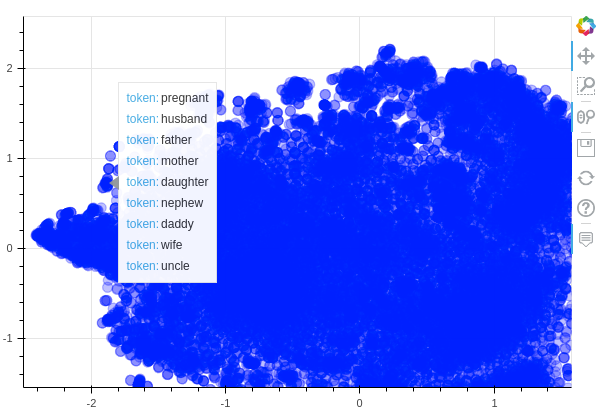
\includegraphics[scale=0.75]{pics/points.png}
\newpage

  
  \chapter{Предобработка данных}

Машинное обучение является мощным и эффективным инструментом при реализации
алгоритмов классификации, маршрутизации, обработки и поиска документов, однако, определяющее значение в этих процессах имеет качество исходных данных \cite{bib2}. Именно поэтому проведение подготовки исходных документов, их предварительная обработка позволяет значительно повысить точность результатов, получаемых в ходе применения
машинного обучения. 


\section{Тематическое моделирование}

Тематическая модель (англ. \textit{topic model}) — модель коллекции текстовых документов, которая определяет, к каким темам относится каждый документ коллекции. Алгоритм построения тематической модели получает на входе коллекцию текстовых документов. На выходе для каждого документа выдаётся числовой вектор, составленный из оценок степени принадлежности данного документа каждой из тем. Размерность этого вектора, равная числу тем, может либо задаваться на входе, либо определяться моделью автоматически.

Тематическое моделирование (англ. \textit{topic modeling}) — построение тематической модели.

Задача построения тематической модели звучит следующим образом. Задана коллекция текстовых документов $D$. Каждый документ $d$ из коллекции $D$ представляет собой последовательность слов $W_d=(w_1,\ldots,w_{n_d})$ из словаря $W$, где $n_d$ — длина документа $d$. Предполагается, что каждый документ может относиться к одной или нескольким темам. Темы отличаются друг от друга различной частотой употребления слов. Требуется найти эти темы, то есть определить
\begin{itemize}
\item число тем;
\item распределения частот слов, характерное для каждой темы;
\item тематику каждого документа — в какой степени он относится к каждой из тем.
\end{itemize}

Данная задача может рассматриваться как задача одновременной кластеризации документов и слов по одному и тому же множеству кластеров, называемых темами. Строится, так называемая, мягкая кластеризация, то есть один документ может принадлежать нескольким темам в различной степени.

Для тематического моделирования в качестве модели в данной работе используется латентное размещение Дирихле (англ. \textit{latent Dirichlet allocation, LDA}) \cite{bib4}.

Для оценки качества данной модели используется перплексия (англ. \textit{perplexity}) --- оценка того, насколько хорошо вероятностная модель предсказывает выборку. Низкая перплексия указывает на то, что распределение вероятностей хорошо предсказывает выборку. 

В зависимости от параметра модели, отвечающего за количество тем у распределения текстов, получилась следующая зависимость значения перплексии от количества тем:

\includegraphics[scale=0.5]{pics/perplexity.png}

Ниже приведены примеры слов, принадлежащие каждой из 6 (с оптимальным значением перплексии) тем:

\begin{tabular}{ | l | l | l | }
\hline
Номер темы & Слова \\ \hline
1 & obama, state, president, government, american, \\ & israel,  policy, country \\ \hline
2 & woman, say, work, health, year, senate, group, \\ & government,  support, company \\ \hline
3 & call, get, work, see, want, know, good, also, think, tomorrow \\ \hline
4 & secretary, office, state, meet, room, department,  \\ &  arrive, route, depart, private \\ \hline 
5 & state, information, benghazi, department, doc, case, subject, \\ & iran, agreement, house \\ \hline
6 & cheryl, gov, fyi, sullivan, state, friday, sunday, branch,  \\ & wednesday, april, january \\ \hline 

\end{tabular}

\newpage

Распределение слов по темам:

\includegraphics[scale=0.5]{pics/words_map.png}



\section{Предобработка электронных писем корпорации Enron}

\subsection{Выделение метаданных из сырого текста писем}

Набор данных \textit{Enron} также требует предварительной обработки. К примеру, так выглядит необработная информация одного электронного письма:

\begin{verbatim}
Message-ID: <18782981.1075855378110.JavaMail.evans@thyme>
Date: Mon, 14 May 2001 16:39:00 -0700 (PDT)
From: phillip.allen@enron.com
To: tim.belden@enron.com
Subject: 
Mime-Version: 1.0
Content-Type: text/plain; charset=us-ascii
Content-Transfer-Encoding: 7bit
X-From: Phillip K Allen
X-To: Tim Belden <Tim Belden/Enron@EnronXGate>
X-cc: 
X-bcc: 
X-Folder: \\Phillip_Allen_Jan2002_1\\Allen, Phillip K.\\\'Sent Mail
X-Origin: Allen-P
X-FileName: pallen (Non-Privileged).pst

Here is our forecast
\end{verbatim}

Конечно, анализировать данные (в том числе метаинформацию о письме) в таком формате бессмысленно. Для обработки мы будем использовать библиотеку \textit{email} \cite{bib8}. Данная библиотека позволяет из сырых данных выделить вспомогательную информацию о письме, в частности, библиотека позволяет выделить следующие интересные нам атрибуты:
\begin{itemize}
\item полное содержание письма,
\item дата отправки,
\item адрес получателя,
\item адрес отправителя,
\item тема письма,
\item логин отправителя.
\end{itemize}

\subsection{Выделение содержания писем}

После этого требуется также привести содержание письма в приемлимый для дальнейшего обучения вид. Например, для письма с содержанием ниже мы хотим выделить только единицы, имеющие отношение к сути письма.

\begin{verbatim}

Forwarded by Phillip K Allen/HOU/ECT on 09/12/2000 11:22 AM 

Michael Etringer

09/11/2000 02:32 PM

To: Phillip K Allen/HOU/ECT@ECT
cc:  
Subject: Contact list for mid market

Phillip,
Attached is the list. Have your people fill in the columns 
highlighted in yellow. As best can we will try not to overlap
on accounts. 
Thanks, Mike
\end{verbatim}

Выделение этих единиц происходит в соответствии со следующей последовательности шагов:
\begin{enumerate}
\item Перевод всех символов в нижний регистр.
\item Удаление всех слов, содержащих цифры. Такие слова не несут смысловой нагрузки и, соответственно, влияют на качество обучения в худшую сторону (подавляющее большинство таких слов было получено отправителями по ошибке).
\item Удаление единиц, соответствующих информации о пересланных письмах.
\item Удаление единиц, соответствующих информации о вложениях в письме.
\item Удаление единиц, соответствующих почтовым адресам, присутствующим в тексте писем.
\item Удаление единиц, соответствующих корпоративным именам пользователей.
\item Удаление единиц, соответствующих ссылкам в сети Интернет.
\item Удаление единиц, не несущих смысловой составляющей, в заголовке письма.
\end{enumerate}

Шаги 3-7 выполняются с использованием регулярных выражений. 

В результате, для примера выше, дальнейшая работа будет производиться со следующим текстом:
\begin{verbatim}
contact list for mid market. phillip, attached is the list. 
have your people fill in the columns highlighted in yellow. 
as best can we will try not to overlap on accounts. thanks, mike'
\end{verbatim}



% \section{Тематическое моделирование}

Тематическая модель (англ. \textit{topic model}) — модель коллекции текстовых документов, которая определяет, к каким темам относится каждый документ коллекции. Алгоритм построения тематической модели получает на входе коллекцию текстовых документов. На выходе для каждого документа выдаётся числовой вектор, составленный из оценок степени принадлежности данного документа каждой из тем. Размерность этого вектора, равная числу тем, может либо задаваться на входе, либо определяться моделью автоматически.

Тематическое моделирование (англ. \textit{topic modeling}) — построение тематической модели.

Задача построения тематической модели звучит следующим образом. Задана коллекция текстовых документов $D$. Каждый документ $d$ из коллекции $D$ представляет собой последовательность слов $W_d=(w_1,\ldots,w_{n_d})$ из словаря $W$, где $n_d$ — длина документа $d$. Предполагается, что каждый документ может относиться к одной или нескольким темам. Темы отличаются друг от друга различной частотой употребления слов. Требуется найти эти темы, то есть определить
\begin{itemize}
\item число тем;
\item распределения частот слов, характерное для каждой темы;
\item тематику каждого документа — в какой степени он относится к каждой из тем.
\end{itemize}

Данная задача может рассматриваться как задача одновременной кластеризации документов и слов по одному и тому же множеству кластеров, называемых темами. Строится, так называемая, мягкая кластеризация, то есть один документ может принадлежать нескольким темам в различной степени.

Для тематического моделирования в качестве модели в данной работе используется латентное размещение Дирихле (англ. \textit{latent Dirichlet allocation, LDA}) \cite{bib4}.

Для оценки качества данной модели используется перплексия (англ. \textit{perplexity}) --- оценка того, насколько хорошо вероятностная модель предсказывает выборку. Низкая перплексия указывает на то, что распределение вероятностей хорошо предсказывает выборку. 

В зависимости от параметра модели, отвечающего за количество тем у распределения текстов, получилась следующая зависимость значения перплексии от количества тем:

\includegraphics[scale=0.5]{perplexity.png}

Ниже приведены примеры слов, принадлежащие каждой из 6 (с оптимальным значением перплексии) тем:

\begin{tabular}{ | l | l | l | }
\hline
Номер темы & Слова \\ \hline
1 & obama, state, president, government, american, \\ & israel,  policy, country \\ \hline
2 & woman, say, work, health, year, senate, group, \\ & government,  support, company \\ \hline
3 & call, get, work, see, want, know, good, also, think, tomorrow \\ \hline
4 & secretary, office, state, meet, room, department,  \\ &  arrive, route, depart, private \\ \hline 
5 & state, information, benghazi, department, doc, case, subject, \\ & iran, agreement, house \\ \hline
6 & cheryl, gov, fyi, sullivan, state, friday, sunday, branch,  \\ & wednesday, april, january \\ \hline 

\end{tabular}

\newpage

Распределение слов по темам:

\includegraphics[scale=0.5]{words_map.png}


%\section{Предобработка электронных писем корпорации Enron}

\subsection{Выделение метаданных из сырого текста писем}

Набор данных \textit{Enron} также требует предварительной обработки. К примеру, так выглядит необработная информация одного электронного письма:

\begin{verbatim}
Message-ID: <18782981.1075855378110.JavaMail.evans@thyme>
Date: Mon, 14 May 2001 16:39:00 -0700 (PDT)
From: phillip.allen@enron.com
To: tim.belden@enron.com
Subject: 
Mime-Version: 1.0
Content-Type: text/plain; charset=us-ascii
Content-Transfer-Encoding: 7bit
X-From: Phillip K Allen
X-To: Tim Belden <Tim Belden/Enron@EnronXGate>
X-cc: 
X-bcc: 
X-Folder: \\Phillip_Allen_Jan2002_1\\Allen, Phillip K.\\\'Sent Mail
X-Origin: Allen-P
X-FileName: pallen (Non-Privileged).pst

Here is our forecast
\end{verbatim}

Конечно, анализировать данные (в том числе метаинформацию о письме) в таком формате бессмысленно. Для обработки мы будем использовать библиотеку \textit{email} \cite{bib8}. Данная библиотека позволяет из сырых данных выделить вспомогательную информацию о письме, в частности, библиотека позволяет выделить следующие интересные нам атрибуты:
\begin{itemize}
\item полное содержание письма,
\item дата отправки,
\item адрес получателя,
\item адрес отправителя,
\item тема письма,
\item логин отправителя.
\end{itemize}

\subsection{Выделение содержания писем}

После этого требуется также привести содержание письма в приемлимый для дальнейшего обучения вид. Например, для письма с содержанием ниже мы хотим выделить только единицы, имеющие отношение к сути письма.

\begin{verbatim}

Forwarded by Phillip K Allen/HOU/ECT on 09/12/2000 11:22 AM 

Michael Etringer

09/11/2000 02:32 PM

To: Phillip K Allen/HOU/ECT@ECT
cc:  
Subject: Contact list for mid market

Phillip,
Attached is the list. Have your people fill in the columns 
highlighted in yellow. As best can we will try not to overlap
on accounts. 
Thanks, Mike
\end{verbatim}

Выделение этих единиц происходит в соответствии со следующей последовательности шагов:
\begin{enumerate}
\item Перевод всех символов в нижний регистр.
\item Удаление всех слов, содержащих цифры. Такие слова не несут смысловой нагрузки и, соответственно, влияют на качество обучения в худшую сторону (подавляющее большинство таких слов было получено отправителями по ошибке).
\item Удаление единиц, соответствующих информации о пересланных письмах.
\item Удаление единиц, соответствующих информации о вложениях в письме.
\item Удаление единиц, соответствующих почтовым адресам, присутствующим в тексте писем.
\item Удаление единиц, соответствующих корпоративным именам пользователей.
\item Удаление единиц, соответствующих ссылкам в сети Интернет.
\item Удаление единиц, не несущих смысловой составляющей, в заголовке письма.
\end{enumerate}

Шаги 3-7 выполняются с использованием регулярных выражений. 

В результате, для примера выше, дальнейшая работа будет производиться со следующим текстом:
\begin{verbatim}
contact list for mid market. phillip, attached is the list. 
have your people fill in the columns highlighted in yellow. 
as best can we will try not to overlap on accounts. thanks, mike'
\end{verbatim}


%\section{Нахождение начального треугольника}

Для дальнейшего хода алгоритма требуется найти какой-нибудь начальник треугольник, являющийся валидным или частично валидным. Любой треугольник, который содержит хотя бы вершину, принадлежащую выпуклой оболочке всех вершин исходной сетки, является валидным или частично валидным и подойдет нам как начальный треугольник. На самом деле можно поступить еще проще, если заметить, что среди треугольников, которые касаются $AABB$ исходной сетки, можно найти валидный и соответственно выбрать его в качестве начального.
%\section{Построение \textit{валидной области}}

Для нахождения \textit{валидной области}, мы используем подход, использующий начальный треугольник, найденный ранее.
Также, вместо того, чтобы заранее разбивать все пересекающиеся треугольники, мы будем разбивать только те частично валидные треугольники, которые появлялись в ходе работы дальнейшего алгоритма, чтобы не совершать лишние операции над невалидными треугольниками. Подробнее, алгоритм построения \textit{валидной области} состоит из следующих шагов:

\begin{enumerate}
\item
Каждый треугольник может иметь одно из следующих состояний:
\begin{itemize}
\item непосещенный треугольник,
\item валидный треугольник,
\item частично валидный треугольник.
\end{itemize}
Изначально все треугольники помечаются как непосещенные.

\item
Начальный треугольник, найденный ранее, помечается валидным и добавляется в некоторое множество $\mathbf{S}$.

\item
Если множество $\mathbf{S}$ пусто, перейти к пункту 5. Иначе, достать треугольник $T$ из $\mathbf{S}$.

\item
Для каждого непосещенного треугольника $T_a$, смежного с $T$, если $T_a$ не пересекается с другими треугольниками, он добавляется в $\mathbf{S}$. В противном случае, $T_a$ помечается частично валидным и добавлется в другое множество $\mathbf{P}$. $T_a$ добавляется в $\mathbf{P}$ вместе с информацией о ребре $e_p$, которое являлось смежным для $T$ и $T_a$.

\item
Если множество $\mathbf{P}$ пусто, перейти к пункту 7. Иначе, достать частично валидный треугольник $T_p$ и его ребро $e_p$ из $\mathbf{P}$.

\item
Триангулировать $T_p$ (детали в секции 2.5). Продолжить построение \textit{валидной области} с помощью $T_p$ и его подтреугольников (как описано в секции 2.6). Если другой начальный треугольник найден, он добавляется в $\mathbf{S}$ и нужно перейти к пункту 2. Иначе, перейти к пункту 4.

\item Построение \textit{валидной области} завершено.

\end{enumerate}


%\section{Триангуляция}

Частично валидный треугольник $T_p$ имеет некоторое количество отрезков пересечений с другими треугольниками. Триангуляция на этом шаге выполняется для того, чтобы: (1) разделить $T_p$ на подтреугольники, которые содержат отрезки пересечений в качестве своих сторон, (2) продолжить построение внутри сетки из полученных подтреугольников.

Подробнее, шаги для (1) следующие:

\begin{enumerate}
\item Разделить каждую сторону треугольника $T_p$ всеми отрезками пересечений $\{s_i\}$.
\item Разделить каждый $s_i$ всеми другими отрезками пересечений.
\item Триангулировать $T_p$ с помощью двумерной триангуляции Делоне с ограничениями (\textit{2D constrained Delaunay triangulation}) \cite{triangulation} вместе со сторонами треугольника и отрезками пересечений, полученных в $1$ и $2$.

\end{enumerate}
Для полученных подтреугольников, дальнеший алгоритм построения начинается с ребра $e_p$. Подтреугольник, смежный ребру $e_p$ помечается валидным и становится начальным для процесса построения в подтреугольниках. Затем валидная часть $T_p$ распространяется к соседним подтреугольникаам до тех пор, пока не достигнет ребер, являющихся частью отрезков пересечений, которые играют роль ребер-входов в соседние треугольники $T_c$ для следующего шага, описанного в секции 2.6.



%\section{<<Crossing the river>>}

\begin{figure}[h]
  \label{fig:cross}
  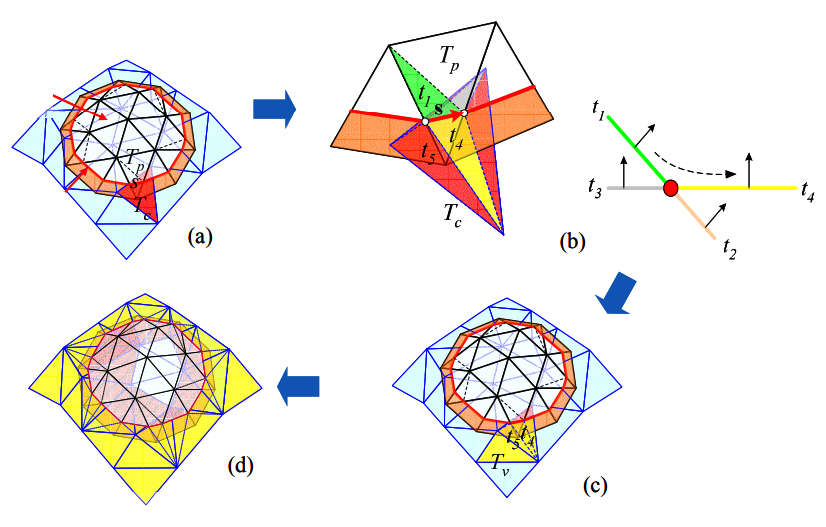
\includegraphics[width=0.7\linewidth]{36.png}
  \centering
  \caption{подробные шаги <<crossing the river>>}
\end{figure}

Процесс построения \textit{валидного региона} может распространиться за самопересечение и переместиться к подтреугольникам соседнего треугольника. Рисунок $2.1$ иллюстрирует подробные шаги распространия внутри подтреугольников частично валидного треугольника. Все начинается с триангуляции соседнего треугольника $T_c$ как в секции 2.5. На рисунке (b) есть два треугольника $t_3$, $t_4$, смежных с ребром-входом. Подтреугольник $t_4$ выбирается как валидный, и будет служить как начальный треугольник в процессе построения внутри подтреугольников $T_c$. В конце концов, как показано на рисунке (c), треугольник $T_v$ будет найден как валидный треугольник и будет добавлен в $\mathbf{S}$.



%\section{<<Сшивание>>}

Так как все частично валидные треугольник были заменены на подтреугольники, а все валидные треугольники уже помечены, в конце нужно оставить только валидные треугольники, а все остальные игнорировать. После этого нужно <<сшить>> ребра самопересечений, определив, что соответствеющие смежные ребра связаны.
  
  \chapter{Предварительный анализ электронных писем}

Прежде чем приступать к исследованию данных методами машинного обучения, может быть полезно посмотреть на различного статистики.

\section{Анализ электронных писем Хиллари Клинтон}

\subsection{Количества слов}

\begin{itemize}

\item Гистограмма распределения количества слов каждой длины: 

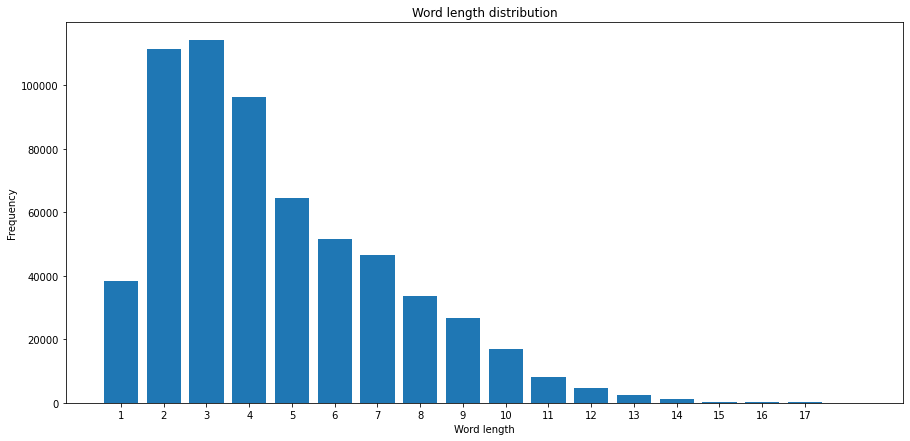
\includegraphics[scale=0.5]{pics/word_lengths.png}

Гистограмма выглядит вполне естественным образом, много коротких слов (например, местоимений, предлогов).

\item Гистограмма распределения длин (в количестве слов) писем:

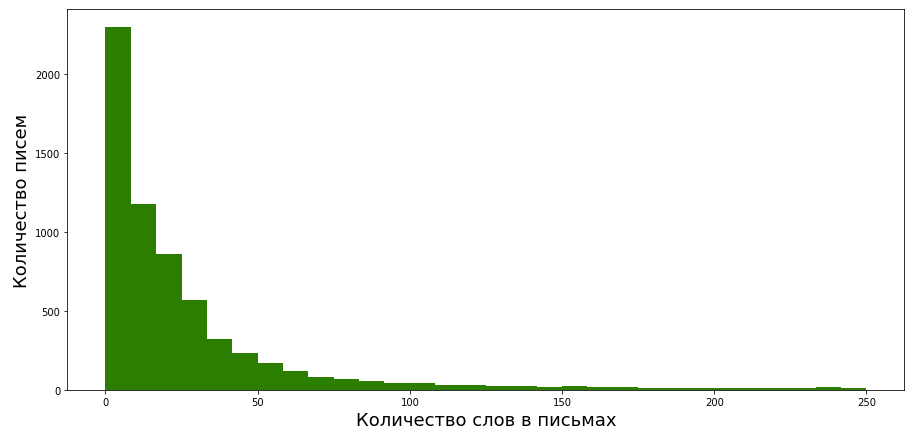
\includegraphics[scale=0.5]{pics/email_lengths.png}

Гистограмма соответствует интуитивным ожиданиям -- более длинные письма пишутся реже. 
\end{itemize}

\subsection{Время отправки писем}

\begin{itemize}

\item Количество отправленных писем по годам:

$ $

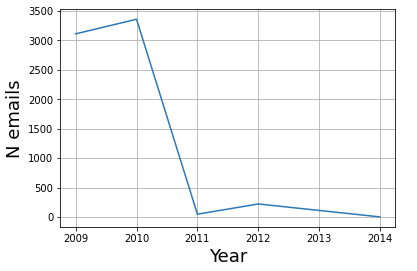
\includegraphics[scale=0.8]{pics/year.png}

На графике можно заметить странную аномалию с нулем писем в 2011 году. Вероятнее всего, это связано с особенностями набора данных. 

\item Количество отправленных писем по дням недели:

$ $

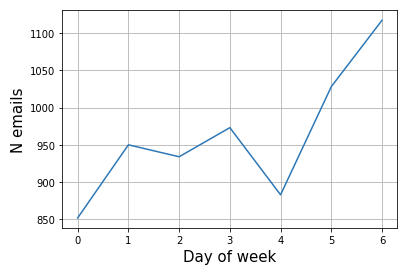
\includegraphics[scale=0.8]{pics/week.png}

График выглядит слегка неестественно (в отличие от \textit{Enron}). Можно попытаться интерпретировать это как особенности одного отдельного человека, занимающего специфичным видом деятельности.
\end{itemize}


\section{Анализ электронных писем корпорации Enron}

\subsection{Длины писем}

Гистограмма распределения длин (в количестве слов) писем:

$ $

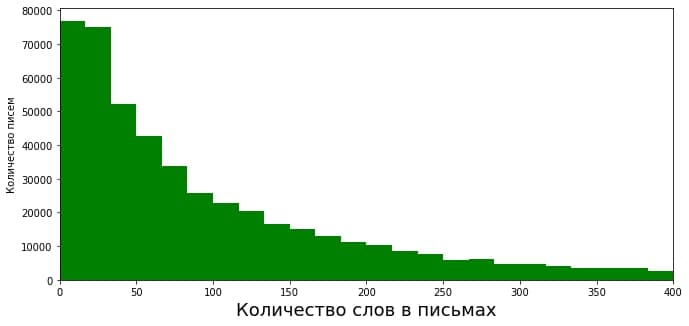
\includegraphics[scale=0.75]{pics/enron_emails_words_count.jpg}

Гистограмма, как и в случае писем Клинтон, соответствует интуитивным ожиданиям -- более длинные письма пишутся реже. 

\subsection{Время отправки писем}

\begin{itemize}

\item Количество отправленных писем по годам:

$ $

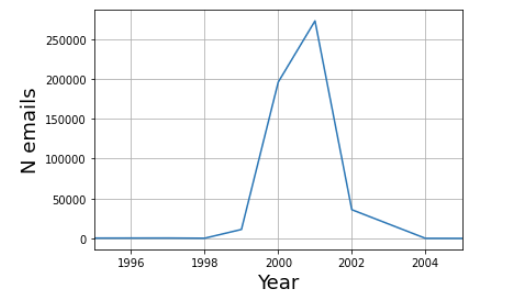
\includegraphics[scale=0.8]{pics/enron_year.png}

График соответствует наибольшей активности компании в 2000-2001 годах и банкротству к концу 2001 года.

\item Количество отправленных писем по дням недели:

$ $

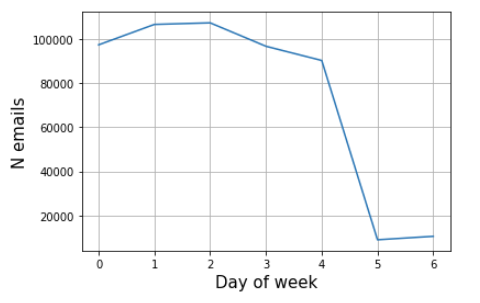
\includegraphics[scale=0.8]{pics/enron_week.png}

Этот график также выглядит естественно --- наибольшее число писем во вторник и среду, в середине рабочей недели, наименьшее --- в выходные дни.

\item Количество отправленных писем по времени суток:

$ $

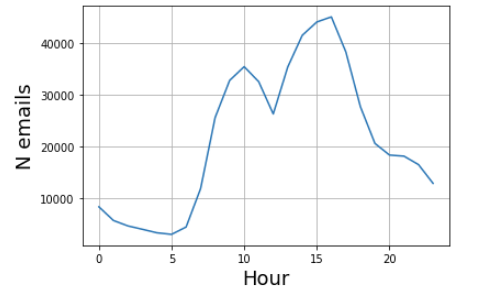
\includegraphics[scale=0.8]{pics/enron_hour.png}

На графике вышем видим наибольшую продуктивность во вторую половину дня, низкую активность в ночные часы, а также аномалию в самом разгаре дня, объсняющуюся обеденным перерывом.

\end{itemize}

\subsection{Частотность слов}

Для интерпретации самых часто используемых слов использовались так называемые облака слов.

Облако слов -- это метод визуализации данных, используемый для представления текстовых данных, в которых размер каждого слова указывает его частоту или важность. Важные точки текстовых данных могут быть выделены с помощью облака слов. Облака слов широко используются для анализа данных с веб-сайтов социальных сетей.


\begin{itemize}
\item Облако слов, построенное по словам из тем электронных писем:

\begin{center}
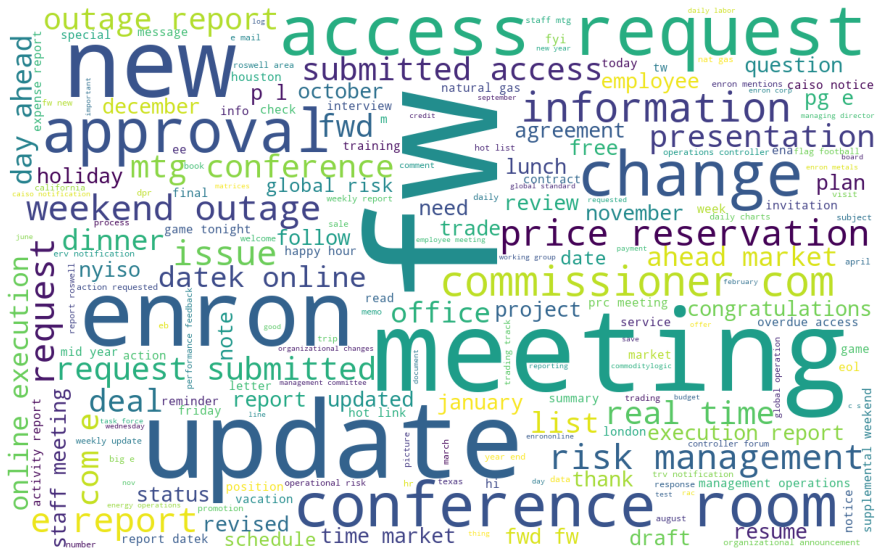
\includegraphics[scale=0.5]{pics/enron_wordcloud_subject.png}
\end{center}

Слова, встречающиеся в темах писем: \texttt{meeting}, \texttt{conference room}, \texttt{update}, \texttt{approval},\texttt{access request}, \texttt{enron}.

\item Облако слов, построенное по словам из содержания электронных писем:

\begin{center}

\includegraphics[scale=0.5]{pics/enron_wordcloud_content.png}
\end{center}

Слова, встречающиеся в содержании писем: \texttt{enron}, \texttt{week}, \texttt{thank}, \texttt{know}, \texttt{new}.

\end{itemize}

\subsection{Отправители и получатели писем}

\begin{itemize}
\item 20 адресов, с которых было отправлено наибольшее количество электронных писем:

\begin{center}
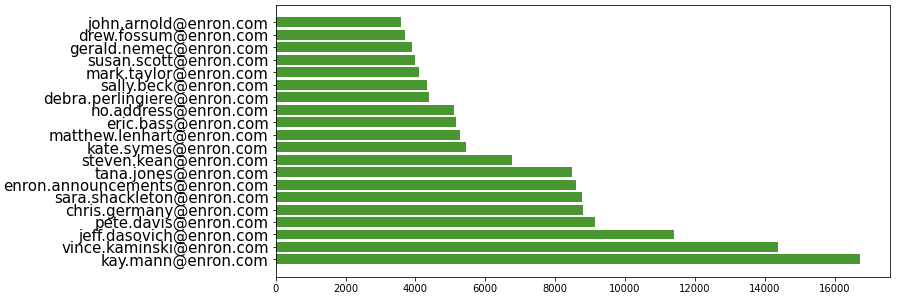
\includegraphics[scale=0.5]{pics/enron_most_sent.png}
\end{center}

\item 20 адресов, на которые было отправлено наибольшее количество электронных писем:

\begin{center}
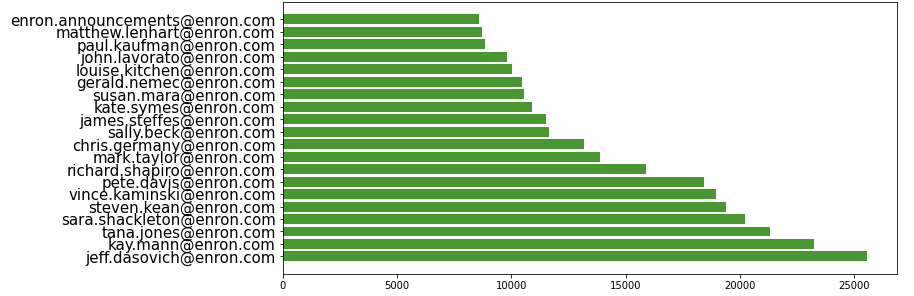
\includegraphics[scale=0.5]{pics/enron_most_recieved.png}
\end{center}

Как видим, в графиках распределения получателей и отправителей писем много различий --- некоторые люди пишут писем меньше, чем получают и наоборот.

\item Теперь посмотрим количество писем между фиксированной парой собеседников. Рассмотрим только электронные письма, отправленные на один адрес электронной почты, так как они могут быть более важными личными сообщениями.

\begin{center}
\begin{tabular}{ | l | l | l | }
\hline
Отправитель & Получатель & Количество \\ \hline
pete.davis & pete.davis & 9141 \\ \hline
vince.kaminski & vkaminski@aol.com & 4308 \\ \hline
enron.announcements & all.worldwide & 2206 \\ \hline
enron.announcements & all.houston & 1701 \\ \hline
kay.mann & suzanne.adams & 1528 \\ \hline
vince.kaminski & shirley.crenshaw & 1190 \\ \hline
steven.kean & maureen.mcvicker & 1014 \\ \hline
kay.mann & nmann@erac.com	 & 980 \\ \hline
kate.symes & evelyn.metoyer & 	915 \\ \hline
kate.symes & kerri.thompson	 & 859 \\ \hline
\end{tabular}
\end{center}

Здесь интересно, что некоторые люди отправляют сами себе много электронных писем.


\end{itemize}

\newpage


\begin{thebibliography}{3}

\bibitem{bib234234}
BERTopic. \url{https://maartengr.github.io/BERTopic/}.

\bibitem{bib_1}
Jacob Devlin, Ming-Wei Chang, Kenton Lee, Kristina Toutanova. BERT: Pre-training of Deep Bidirectional Transformers for Language Understanding. 
\url{https://arxiv.org/abs/1810.04805}.

\bibitem{bib_2}
Lena Voita. 
(Introduction to) Transfer Learning. \url{https://lena-voita.github.io/nlp_course/transfer_learning.html}.

\bibitem{bib_3}
Brendan Bailey. Lightning Talk: Clustering with HDBScan. \url{https://towardsdatascience.com/lightning-talk-clustering-with-hdbscan-d47b83d1b03a}.

\bibitem{bib1}
Hillary Clinton's Emails,
\url{https://www.kaggle.com/kaggle/hillary-clinton-emails}.

\bibitem{bib2}
Обухов А. Д. Постановка задачи структурно-параметрического синтеза системы
электронного документооборота научно-образовательного учреждения // Вестник ТГТУ. –
2016. – № 2. – С. 217–232. – DOI: 10.17277/
vestnik.2016.02.pp.217-232.

\bibitem{bib3}
Библиотека spaCy. \url{https://spacy.io/}.

\bibitem{bib4}
David M. Blei, Andrew Ng, Michael Jordan. Latent Dirichlet allocation // Journal of Machine Learning Research (3) 2003 pp. 993-1022.

\bibitem{bib5}
Mikolov T., Chen K., Corrado G., Dean J. Efficient Estimation of Word Representations in Vector Space // In Proceedings of Workshop at ICLR. — 2013a.

\bibitem{bib6}
GloVe: Global Vectors for Word Representation. \url{https://nlp.stanford.edu/projects/glove/}.

\bibitem{bib7}
van der Maaten L.J.P., Hinton G.E. Visualizing Data Using t-SNE // Journal of Machine Learning Research. — 2008. — Ноябрь (т. 9).

\bibitem{bib8}
Email — An email and MIME handling package. \url{https://docs.python.org/3/library/email.html}.

\end{thebibliography}


\addcontentsline{toc}{chapter}{Литература}


  % \section{Первый нумерованный раздел}
  % \label{s:first_num_sec}

  

  % \blindmathpaper
  % \subsection{Первый нумерованный подраздел}
  % \label{ss:first_num_subsec}
  % \blindmathpaper

  % \chapter{Вторая нумерованная глава}
  % \label{c:second_num_chap}
  % \blindmathpaper
  % \section{Второй нумерованный раздел}
  % \label{s:second_num_sec}
  % \blindmathpaper
  % \subsection{Второй нумерованный подраздел}
  % \label{ss:second_num_subsec}
  % \blindmathpaper

  % \appendix
  % \section{Один}
  % \blindmathpaper
  % \section{Два}
  % \blindmathpaper
  % \section{Три}
  % \blindmathpaper

  % \lstinputlisting[language=R, caption=Исходный кот, label=lst:code]{code.R}

\end{document}